% Introduction
\subsection{Introduction}
In the two decades since \glspl{FPGA} were introduced, they have radically
changed the way digital logic is designed and deployed \cite{Hauck:2007}.
\glspl{FPGA} are revolutionary devices that offer a compromise between the
flexibility and ease of microprocessor-based software designs; and the
performance and efficiency of \gls{ASIC}-based hardware design. Unlike an
\gls{ASIC}, computations are programmed into the \gls{FPGA} device, instead of
being permanently constructed during the manufacturing process. This means that
an \gls{FPGA} device can be programmed and reprogrammed ny times, allowing for
a significant level of flexibility whilst enabling a much faster and efficient
implementation than a software equivalent.

These benefits, however, do not come without a cost. Designing an
\gls{FPGA}-based system is a more complicated process than the development of a
software process. In order to effectively utilise hardware resources, the
designer of an \gls{FPGA}-based system must consider the hardware resources that
are provided by the \gls{FPGA} device, and must remain flexible during the
design process so as to utilise as many of the hardware resources that are
available whilst ensuring that the highest level of performance is obtained.
These considerations are seldom necessary in a pure-software approach, as tools
such as compilers and assemblers abstract the hardware implementation details
away from the developers in order to provide cross-system and, often,
cross-architecture compatability.

Compared to an \gls{ASIC} design, which may take many months or years to design
and have a multimillion-dollar price tag, an \gls{FPGA} design might only take
days to create and cost tens to hundreds of dollars \cite{Hauck:2007}.

\begin{figure}
    \centering
    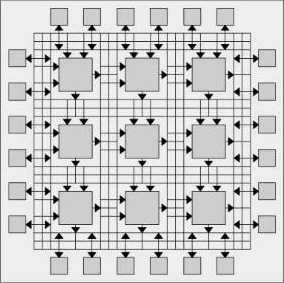
\includegraphics[width=0.5\textwidth]{fpga/abstract-view}
    \caption[An abstract view of an \gls{FPGA}.]
        {An abstract view of an \gls{FPGA} \cite{Hauck:2007}.}
    \label{fig:fpga:abstract}
\end{figure}
